%%%%%%%%%%%%%%%%%%%%%%%%%%%%%%%%%%%%%%%%%%%%%%%%%%%%%%%%%%%%%%%%%%%%%%%%%%%%%%%%%%%%%%%%%%%%%%%%%%%%%%%%%%
%%%   %%%%
%%%%%%%%%%%%%%%%%%%%%%%%%%%%%%%%%%%%%%%%%%%%%%%%%%%%%%%%%%%%%%%%%%%%%%%%%%%%%%%%%%%%%%%%%%%%%%%%%%%%%%%%%%%

\documentclass[runningheads,a4paper]{llncs}

\usepackage[utf8]{inputenc}
\usepackage{amssymb}
\setcounter{tocdepth}{3}
\usepackage{graphicx}
\usepackage{tabularx}
\usepackage{url}
\usepackage{listings}
\usepackage{subfigure}
\usepackage{algorithmic}
\usepackage{algorithm}

\newcommand{\keywords}[1]{\par\addvspace\baselineskip
\noindent\keywordname\enspace\ignorespaces#1}

% todo macro
\usepackage{color}
\newtheorem{deflda}{Axiom}
\newcommand{\todo}[1]{\noindent\textcolor{red}{{\bf \{TODO}: #1{\bf \}}}}

% Language Definitions for Turtle
\definecolor{olivegreen}{rgb}{0.2,0.8,0.5}
\definecolor{grey}{rgb}{0.5,0.5,0.5}
\lstdefinelanguage{ttl}{
sensitive=true,
morecomment=[l][\color{brown}]{@},
morecomment=[l][\color{red}]{\#},
morestring=[b][\color{blue}]\",
}

%%%%%%%%%%%%%%%%%%%%%%%%%%%%%%%
%%%  Beginning of document  %%%
%%%%%%%%%%%%%%%%%%%%%%%%%%%%%%%

\begin{document}

% first the title is needed

\title{The Prot{\'e}g{\'e}LOV Plugin: Ontology Access and Reuse for Everyone }


\author{ Nuria Garcia\inst{1}, Ghislain Auguste Atemezing\inst{2}, Boris Villaz{\'o}n Terrazas \inst{1}}

\institute{
Expert System Iberia, Campo de las Naciones, Madrid, Spain. \\
\and MONDECA, 35 boulevard de Strasbourg, Paris, France .\\
\email{<lastname.firstname@eurecom.fr> \\
}
}  

	


\maketitle

%%%%%%%%%%%%%%%%%%
%%%  Abstract  %%%
%%%%%%%%%%%%%%%%%%

\begin{abstract}
Here goes the abstract in less than 200 words.

\keywords{Plugin, ontology engineering, LOV, Prot{\'e}g{\'e}} 
\end{abstract}

%%%%%%%%%%%%%%%%%%%%%%%%%
%%%  1. Introduction  %%%
%%%%%%%%%%%%%%%%%%%%%%%%%

\section{Introduction}\label{sec:introduction}

Prot{\'e}g{\'e} is one the popular framework for developing ontologies in a variety of formats including OWL, RDF(S), and XML Schema. It is backed by a strong community of developers and users in many domains. One success on Prot{\'e}g{\'e} also lies on the availability to extend the core framework adding new functionalities by means of plug-ins.

At the same time, the recent success of Linked Open Vocabularies (LOV) as a central point for curated catalog of ontologies is helping to convey on best practices to publish vocabularies on the Web, as well as to help in the Data publication activity on the Web. LOV comes with many features, such as an API, a search function and a SPARQL endpoint.
 
We propose in this paper to explore, design and implement a plug-in of LOV in Prot{\'e}g{\'e} for easing the development of ontologies by reusing existing vocabularies. 
The tool has to improve the modeling and reuse of ontologies used in the LOD cloud, by providing the following features in Prot{\'e}g{\'e}:

\begin{itemize}
\item Import easily vocabularies from LOV into Prot{\'e}g{\'e}. 
\item Propose to the user a list of candidate vocabularies in LOV matching the term
\item Have an updating mechanism (synchronization) to LOV catalog
\item Check if a new vocabulary created in Prot{\'e}g{\'e} satisfied the LOV recommendations

\item Suggest to LOV a new created vocabulary within Prot{\'e}g{\'e}.
\end{itemize}



%%%%%%%%%%%%%%%%%%%%%%%%%%%%%%%%%%%%%%%%%%%%%%%%%%%%%%%%%%%%%%%%%
%%%  2. Related work  %%%
%%%%%%%%%%%%%%%%%%%%%%%%%%%%%%%%%%%%%%%%%%%%%%%%%%%%%%%%%%%%%%%%%



\section{Related Work}
\label{sec:soa}

Show here some work related to plugin for helping in ontology developement:Neon and other


\section{Linked Open Vocabulaires (LOV)}
\label{sec:lov}

Talk about the LOV catalog and APIs..


%%%%%%%%%%%%%%%%%%%%%%%%%%%%%%%%%%%%%%%%%%%%%%%%%%%
%%%  3.ProtegeLOV Description  %%%
%%%%%%%%%%%%%%%%%%%%%%%%%%%%%%%%%%%%%%%%%%%%%%%%%%%

\section{Prot{\'e}g{\'e}LOV}
\label{sec:classification}
Explain our implementations.. views, controllers\\
Add a screenshot

\begin{figure}
\center
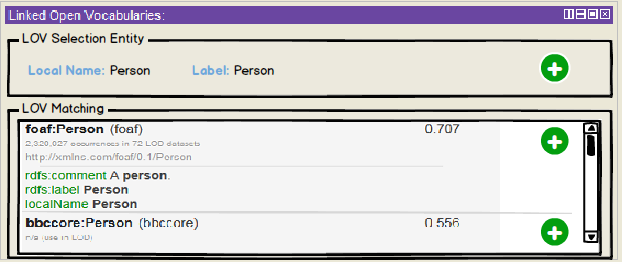
\includegraphics[scale=0.7]{LOVmockup.png}
\end{figure}


%%%%%%%%%%%%%%%%%%%%%%%%%%%%%%%%%%%%%%%
%%%  4. Conclusion and Future Work  %%%
%%%%%%%%%%%%%%%%%%%%%%%%%%%%%%%%%%%%%%%

\section{Evaluation and Future Work}
\label{sec:conclusion}
Small evaluation with few users? and compare with NeOn plugin maybe.


%%%%%%%%%%%%%%%%%%%%%%%%%
%%%  Acknowledgments  %%%
%%%%%%%%%%%%%%%%%%%%%%%%%

\paragraph{\textbf{Acknowledgments.}} %\label{sec:acknowledgments}
Thanks to Pierre-Yves and the LOV team for providing and maintaining a curated vocabularies and API access.
% More acknowledgments here

\bibliographystyle{abbrv}
\nocite{*}
\bibliography{eswcbib}
\end{document}
